\section{Das Projekt}

\subsection*{}
\begin{frame}{Orchestrierung von Webservices}
	
\begin{center}

\includegraphics[width=\textheight]{Bilder/titel_einfuehrung_logos.png} 
\end{center}

\end{frame}

\subsection*{}
\begin{frame}{Die Aufgabenstellung}
\begin{itemize}
	\item \textbf{Datenmigration:} Kontakte von SAP zu Google übertragen
	\pause
	\item \textbf{Strategie:} nicht einfach alle kopieren $\rightarrow$ Karteileichen
		\begin{itemize}
			\item Kontakte nur bei Bedarf übertragen!
			\pause
			\item zunächst bei Google anfragen
			\item erst dann Migration von SAP
			\item sonst manuelle Eingabe
		\end{itemize}
	\pause
	\item \textbf{erste Überlegungen:}
		\begin{itemize}
			\item Aufteilung in drei Bereiche: Google, SAP, SIBs
			\item GUI Elemente für Dateingabe notwendig
		\end{itemize}

\end{itemize}
\end{frame}



\begin{frame}{Projekt-Struktur}
	
\begin{center}
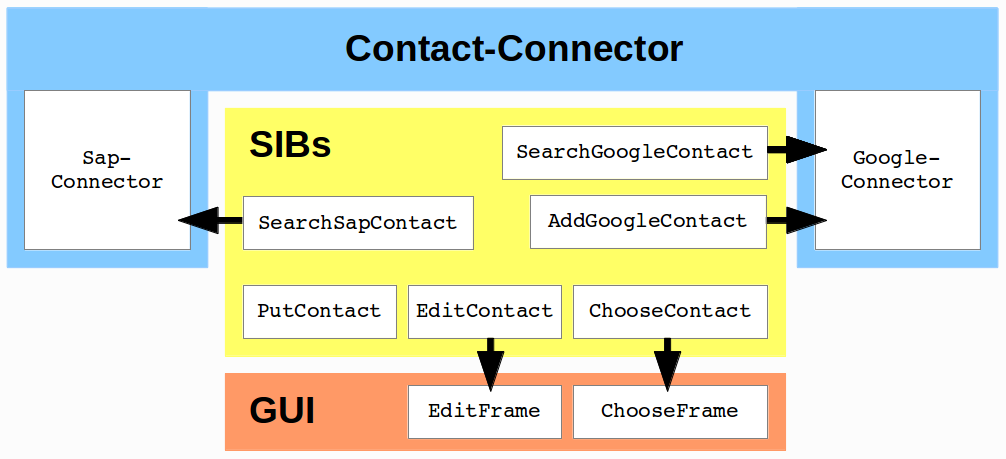
\includegraphics[width=\textheight]{Bilder/projekt_aufbau.png} 
\end{center}

\end{frame}


\subsection*{}
\begin{frame}{Eingesetzte Tools}
\begin{itemize}
	
	\item \textbf{Grundlage:} automatisierte Tests (JUnit), Versionsverwaltung (git)
	\pause
	\item \textbf{Apache Maven:} Build-Management-Tool
		\begin{itemize}
			
			\item unterstützt Software-Lebenszyklus $\rightarrow$ automatische Ausführung der Tests
			\item einfaches Einbinden von Abhängigkeiten (externe Pakete)
			\item verpackt alle Komponenten zu einer JAR-Datei $\rightarrow$ jABC-Projekt
		\end{itemize}
\end{itemize}

\end{frame}











